%%%%%%%%%%%%%%%%%%%%%%%%%%%%%%%%%%%%%%%%%%%%%%%%%%%%%%%%%%%%%%%%%%%%%%%%%%%%%%%%
%2345678901234567890123456789012345678901234567890123456789012345678901234567890
%        1         2         3         4         5         6         7         8
% DOCUMENT CLASS
\documentclass[oneside,12pt]{Classes/RoboticsLaTeX}

% USEFUL PACKAGES
% Commonly-used packages are included by default.
% Refer to section "Book - Useful packages" in the class file "Classes/RoboticsLaTeX.cls" for the complete list.
\usepackage{amsmath}
\usepackage{amsfonts}
\usepackage{algorithm}
\usepackage{algorithmic}
\usepackage{lettrine}

% SPECIAL COMMANDS
% correct bad hyphenation
\hyphenation{op-tical net-works semi-conduc-tor}
%% ignore slightly overfull and underfull boxes
%\hbadness=10000
%\hfuzz=50pt
% declare commonly used operators
\DeclareMathOperator*{\argmax}{argmax}

% OPTIONS
\hypersetup{colorlinks=true, linkcolor=blue, citecolor=blue}

% HEADER
\ifpdf
    \pdfinfo {/Title (Cooperative Assembly for Mobile Manipulators in an Underwater Mission Scenario)
              /Creator (TeX)
              /Producer (pdfTeX)
              /Author (Davide Torielli)
              /CreationDate (D:20190110182500) %format D:YYYYMMDDhhmmss
              /ModDate (20190110182500)
              /Subject (Cooperative Assembly for Mobile Manipulators in an Underwater Mission Scenario)
              /Keywords (Thesis, Underwater, TPIK, Mobile Manipulators, Cooperative manipulators, cooperative assembly, AUV, UVMS, Peg-in-hole)}
    \pdfcatalog {/PageMode (/UseOutlines)
                 /OpenAction (fitbh) }
\fi

\title{Cooperative Assembly for Mobile Manipulators in an Underwater Mission Scenario}

\ifpdf
  \author{\href{mailto:toridebraus@gmail.com}{Davide Torielli}}
  \collegeordept{\href{http://www.dibris.unige.it}{DIBRIS - Department of Computer Science, Bioengineering, Robotics and System Engineering}}
  \university{\href{http://www.unige.it}{University of Genova}}
  \crest{
\includegraphics[width=30mm]{logo_unige}}
\else
  \author{Davide Torielli}
  \collegeordept{DIBRIS - Department of Computer Science, Bioengineering, Robotics and System Engineering}
  \university{University of Genova}
  \crest{
\includegraphics[width=30mm]{logo_unige}}
\fi

% DECLARATION
% Use the following command to change the declaration text:
%\renewcommand{\submittedtext}{INSERT NEW TEXT HERE}
\degree{Robotics Engineering}
\degreedate{Semptember, 2019}

%%%%%%%%%%%%%%%%%%%%%%%%%%%%%%%%%%%%%%%%%%%%%%%%%%%%%%%%%%%%%%%%%%%%%%%%%%%%%%%%

\begin{document}

% A page with the abstract and running title and author etc may be
% required to be handed in separately. If this is not so, comment
% the following 3 lines:
% \begin{abstractseparate}
%   %%%%%%%%%%%%%%%%%%%%%%%%%%%%%%%%%%%%%%%%%%%%%%%%%%%%%%%%%%%%%%%%%%%%%%%%%%%%%%%%
%2345678901234567890123456789012345678901234567890123456789012345678901234567890
%        1         2         3         4         5         6         7         8
% THESIS ABSTRACT

% Use the following style if the abstract is long:
%\begin{abstractslong}
%\end{abstractslong}


\newgeometry{top=2.6cm}
\begin{abstracts}

Robotics is spreading in all the relevant sectors of the human life. The importance of studying this field is confirmed by all the various applications where robots are used: exploration of space and sea, industry, healthcare, transportation and so on. This thesis aims to improve the current state of the art in a particular field: Underwater Robotics. Currently, the research in this area focuses on improving robots capabilities to make them more and more efficient in performing missions autonomously. A particular advancement is towards the cooperation between multiple agents. With cooperation the robotics systems can perform more and more difficult tasks, such as carrying a long and heavy object in an unstructured environment.\\
Specifically, the problem addressed is an \textit{assembly} one known as the \mbox{\textit{peg-in-hole}} task. In this case, two autonomous manipulators must carry \textit{cooperatively} (at kinematic level) a \textit{peg} and must insert it into an \textit{hole} fixed in the environment. Even if the \textit{peg-in-hole} is a well-known problem, there are no specific studies related to the use of two different autonomous manipulators, especially in underwater scenarios. Among all the possible investigations towards the problem, this work focuses mainly on the kinematic control of the robots. The methods used are part of the Task Priority Inverse Kinematics (TPIK) approach, with a cooperation scheme that permits to exchange as less information as possible between the agents (that is really important being water a big impediment for communication). A force-torque sensor is exploited at kinematic level to help the insertion phase. The results show how the TPIK and the chosen cooperation scheme can be used for the stated problem. The simulated experiments done consider little errors in the hole's pose, that still permit to insert the \textit{peg} but with a lot of frictions and possible stucks. It is shown how can be possible to improve (thanks to the data provided by the force-torque sensor) the insertion phase performed by the two manipulators in presence of these errors.\\
Another part of the thesis deals with computer vision algorithms: a third robot exploits  particular methods to estimate the \textit{hole}'s pose. Different techniques are compared to \textit{detect} and to \textit{track} the \textit{hole}, considering the errors they provide in the pose's estimation.\\
Even if the problem is simplified (due to its complexity), this thesis could help further works. The focus is on the particular problem stated, but the methods and tools exploited can be useful also for other applications, not only underwater-related. 

\end{abstracts}

\restoregeometry
% \end{abstractseparate}

\maketitle

% add an empty page after title page
\newpage\null\thispagestyle{empty}\newpage

% set the number of sectioning levels that get number and appear in the contents
\setcounter{secnumdepth}{3}
\setcounter{tocdepth}{3}

\frontmatter
%%%%%%%%%%%%%%%%%%%%%%%%%%%%%%%%%%%%%%%%%%%%%%%%%%%%%%%%%%%%%%%%%%%%%%%%%%%%%%%%%
%2345678901234567890123456789012345678901234567890123456789012345678901234567890
%        1         2         3         4         5         6         7         8
% THESIS ACKNOWLEDGEMENTS

% Use the following style if the acknowledgements are long:
%\begin{acknowledgementslong}
%\end{acknowledgmentslong}

\begin{acknowledgements}

I would like to thank my mother, my father, and my whole family, without whom I would not be here. I would to thank my sweetheart and my love, Sara (aka Cucurucho) which has always supported me and always will do. She was also really important for reviewing my English.\\
I would like to thank the Spanish lab, IRSLab, especially Javier, whom really help me a lot despite every morning at 10:12 he distracted me with Spanish almuerzos. I would also to thank professors from my home country, Professor Giuseppe Casalino, and Ernico Simetti, my two thesis relators. I want also to remember my Spanish Supervisors, Professor Pedro J Sanz and Professor Raul Marin Prades.\\
I think that I have to thanks also my colleague and friend, Fabio. Also him distracted me a lot with very long telephone calls, anyway they were useful for him to learn something from me =) . \textit{Maybe}, \textit{sometimes} it was also useful for me.\\
Last but not least, I have to thank myself, because I'm great. Bravo Tori.


\end{acknowledgements}

%%%%%%%%%%%%%%%%%%%%%%%%%%%%%%%%%%%%%%%%%%%%%%%%%%%%%%%%%%%%%%%%%%%%%%%%%%%%%%%%%
%2345678901234567890123456789012345678901234567890123456789012345678901234567890
%        1         2         3         4         5         6         7         8
% THESIS DEDICATION

\begin{dedication}


\begin{center}
	\thispagestyle{empty}
	\vspace*{\fill}
		\begin{flushright}
		``Choose a job you love,\\
		and you will never have to work a day in your life'' \\
		\textit{Confucius (\href{https://quoteinvestigator.com/2014/09/02/job-love/}{maybe})}
		
		\end{flushright}
	\vspace*{\fill}
\end{center}

 

\end{dedication}

% ----------------------------------------------------------------------

%%% Local Variables: 
%%% mode: latex
%%% TeX-master: "../thesis"
%%% End: 

%%%%%%%%%%%%%%%%%%%%%%%%%%%%%%%%%%%%%%%%%%%%%%%%%%%%%%%%%%%%%%%%%%%%%%%%%%%%%%%%%
%2345678901234567890123456789012345678901234567890123456789012345678901234567890
%        1         2         3         4         5         6         7         8
% THESIS ABSTRACT

% Use the following style if the abstract is long:
%\begin{abstractslong}
%\end{abstractslong}


\newgeometry{top=2.6cm}
\begin{abstracts}

Robotics is spreading in all the relevant sectors of the human life. The importance of studying this field is confirmed by all the various applications where robots are used: exploration of space and sea, industry, healthcare, transportation and so on. This thesis aims to improve the current state of the art in a particular field: Underwater Robotics. Currently, the research in this area focuses on improving robots capabilities to make them more and more efficient in performing missions autonomously. A particular advancement is towards the cooperation between multiple agents. With cooperation the robotics systems can perform more and more difficult tasks, such as carrying a long and heavy object in an unstructured environment.\\
Specifically, the problem addressed is an \textit{assembly} one known as the \mbox{\textit{peg-in-hole}} task. In this case, two autonomous manipulators must carry \textit{cooperatively} (at kinematic level) a \textit{peg} and must insert it into an \textit{hole} fixed in the environment. Even if the \textit{peg-in-hole} is a well-known problem, there are no specific studies related to the use of two different autonomous manipulators, especially in underwater scenarios. Among all the possible investigations towards the problem, this work focuses mainly on the kinematic control of the robots. The methods used are part of the Task Priority Inverse Kinematics (TPIK) approach, with a cooperation scheme that permits to exchange as less information as possible between the agents (that is really important being water a big impediment for communication). A force-torque sensor is exploited at kinematic level to help the insertion phase. The results show how the TPIK and the chosen cooperation scheme can be used for the stated problem. The simulated experiments done consider little errors in the hole's pose, that still permit to insert the \textit{peg} but with a lot of frictions and possible stucks. It is shown how can be possible to improve (thanks to the data provided by the force-torque sensor) the insertion phase performed by the two manipulators in presence of these errors.\\
Another part of the thesis deals with computer vision algorithms: a third robot exploits  particular methods to estimate the \textit{hole}'s pose. Different techniques are compared to \textit{detect} and to \textit{track} the \textit{hole}, considering the errors they provide in the pose's estimation.\\
Even if the problem is simplified (due to its complexity), this thesis could help further works. The focus is on the particular problem stated, but the methods and tools exploited can be useful also for other applications, not only underwater-related. 

\end{abstracts}

\restoregeometry

\tableofcontents
%\listoffigures
%\printglossary  % Print the nomenclature (WAY TOO COMPLEX FOR ME NOW!)
%\addcontentsline{toc}{chapter}{Nomenclature}

\mainmatter
%%%%%%%%%%%%%%%%%%%%%%%%%%%%%%%%%%%%%%%%%%%%%%%%%%%%%%%%%%%%%%%%%%%%%%%%%%%%%%%%
%2345678901234567890123456789012345678901234567890123456789012345678901234567890
%        1         2         3         4         5         6         7         8
% THESIS INTRODUCTION


% TODO identazioen dopo ogni progetto/paragrafo o no?
\chapter{Introduction}
\label{chap:introduction}
\ifpdf
    \graphicspath{{Introduction/Figures/PNG/}{Introduction/Figures/PDF/}{Introduction/Figures/}}
\else
    \graphicspath{{Introduction/Figures/EPS/}{Introduction/Figures/}}
\fi

Nowadays, different kinds of robot are largely used for underwater missions. A particular type of submarine robot is the Underwater Vehicle Manipulator System (UVMS): an autonomous underwater vehicle (AUV) capable of accomplishing tasks that require a certain level of dexterity, thanks to single or multiple arms.\\
A really innovative field for underwater missions is the analysis of cooperation between multiple agents, which permits to extend their flexibility. Cooperative robots are two or more robots, identical or different, that coordinate themselves autonomously (i.e.\ without human intervention) to accomplish various objectives, from mapping an area to assembling an object.   

This thesis focuses on a totally unexplored environment: cooperative \textit{peg-in-hole} assembly with underwater manipulators. It is part of the TWINBOT project, which is devoted to make a step forward to missions in complex scenarios.\\
The experimental set-up is made up of two I-AUV's Girona 500 underwater vehicles, each one equipped with a CSIP Robot arm5E (4 DOF arm with a parallel yaw gripper). The final goal is to successfully coordinate the robots in such a way that the peg, hold by one manipulator, is inserted correctly in the other piece, hold by the second manipulator.
The work focuses on the kinematic layer, adopting inverse kinematic algorithms based on task's priority (TPIK), although for the peg-in-hole task particular attention must be paid to dynamics interactions. Also the communication problems that arise under the water must be taken into account.  \\
The whole work is divided in two step: 

The first step is to adapt solutions of previous works to pick up, recover and transport the objects using two intervention vehicles. This step is based on previous results from MARIS [\cite{IntroMaris0}], TRIDENT [\cite{AbstractTrident}], and MERBOTS [\cite{AbstractMerbots}] projects.

The step further analyses the peg-in-hole problem, with the aim to solve the assembly task (\textit{M4} milestone of TWINBOT). The chosen strategy divides the problem in two phases: Approaching and Insertion. In the first preliminary tasks are done to prepare the assembly, like aligning correctly the end-effectors of the two manipulators. The second phase explores all the problems inherent to the interaction between the \textit{peg} and the \textit{hole}. The work aims to find a solution to make the robots \textit{cooperate}, understanding the forces exchanged between them while they are assembling the parts.

\section{State of the Art}
Robots have been massively introduced in various fields to help humans in different tasks. Nowadays, there are strategies to use them in underwater environments. A manipulator (robot arm) is considered to be the most suitable tool for executing sub-sea intervention operations. Hence, unmanned underwater vehicles (UUVs), such as remotely operated vehicles (ROVs) and autonomous underwater vehicles (AUVs), are equipped with one or more underwater manipulators.

During the last 20 years, underwater manipulators have been used for many different sub-sea tasks in various fields, for example, underwater archaeology [\cite{IntroApp4}; \cite{IntroApp3}], marine geology [\cite{IntroApp1}; \cite{IntroApp2}], and military applications [\cite{IntroApp5}].

There are many specific tasks where the underwater manipulators are important, from salvage of sunken objects [\cite{IntroSpecApp1}] to mine disposal [\cite{IntroSpecApp2}; \cite{IntroSpecApp3}]. One particular scenario is towards the oil and gas industry, where underwater manipulators are used for pipe inspection, opening and closing valves, drilling, rope cutting [\cite{IntroSpecApp4}], and, in general, to reduced field maintenance and development costs [\cite{IntroSpecApp5}]. A recent survey explored the market related to this technology for oil and gas industry [\cite{IntroSpecApp6}].

\subsection{Previous Works in Underwater Missions}
Since early '90s, research in marine robotics started focusing on the development of underwater vehicle manipulator systems (UVMS). ROVs have been largely used, but they have high operational costs. This is due to the need for expensive support vessels, and highly qualified man power effort. In addition, the pilot which operates the vehicle and the arm experiences heavy fatigue in order to carry out the manipulation task.\\


%first works
For the above reasons, the research started to increase the effort toward augmenting the autonomy level in underwater manipulation. For example, to reduce the operator’s fatigue, some autonomous control features were implemented in work class ROVs [\cite{IntroTeleopRov}]. Another solution is to completely replace ROVs with autonomous underwater vehicles (AUVs).

Some pioneering projects in this field carried out in the '90s. The AMADEUS project [\cite{IntroAMADEUS1}] developed grippers for underwater manipulation [\cite{IntroAMADEUS2}] and studied the problem of dual arm manipulation [\cite{IntroAMADEUS3}].

The UNION project [\cite{IntroUNION}] was the first to perform a mechatronic assembly of an autonomous UVMS.\\


% dopo
Early 2000s showed many field demonstrations. The SWIMMER project [\cite{IntroSwimmer1}] developed a prototype autonomous vehicle to deploy a ROV mounted on an AUV. This permitted to remove the need of long umbilical cables and continuous support by vessels on sea surface.

This work was followed by the ALIVE project [\cite{IntroAlive1}; \cite{IntroAlive2}], that achieved autonomous docking of Intervention-AUV (I-AUV) into to a sub-sea structure not specifically created for AUV use.

The SAUVIM [\cite{IntroSauvim1}; \cite{IntroSauvim2}] project carried out the first autonomous floating underwater intervention. It focused on the searching and recovering of an object whose position was roughly known a priori. Here, the AUV weighted 6 tons, and the arm only 65 kg, so the dynamics of the two subsystems were practically decoupled and the two controllers were separated. The mission consisted in the AUV performing station keeping while the arm was recovering the object.

After SAUVIM, a project called RAUVI [\cite{IntroRauvi}] took a step further. Here, the AUV performed a hook-based recovery in a water tank. Again, the control of the vehicle and the arm was separated, even if the Girona 500 light AUV and the small 4-degrees-of-freedom (DOF) arm used had more similar masses than the ones used in SAUVIM.

A milestone was the TRIDENT project [\cite{IntroTrident1}]. For the first time, the vehicle and the arm were controlled in a coordinated manner [\cite{IntroTrident2}] to recovery a black-box mockup [\cite{IntroTrident4}]. The used task priority solution dealt with both equality and inequality control objectives, although the inequality ones were only-scalar, except for the joint limits. This permitted to perform some manipulation tasks \textit{while} considering also other objectives, for example, keeping the object centred in the camera frame. In this project, only the kinematic control layer (and not also a suitable dynamic one) was implemented.

The PANDORA project [\cite{IntroPandora1}] focused on increasing the autonomy of the robot, by recognizing failures and responding to them. The work combined machine learning techniques [\cite{IntroPandora2}] and a task priority kinematic control approach [\cite{IntroPandora3}]. However it dealt with only equality control objectives, with a specific ad-hoc solution to manage the joint limit inequality task.

The TRIDENT concepts were enhanced within the MARIS project [\cite{IntroMaris0}]. The used task priority framework [\cite{IntroMaris1}] permitted to \textit{activate} and \textit{deactivate} equality/inequality control objectives of any dimension (not only scalar ones). This project also extended the problem to cooperative agents [\cite{IntroMaris2}].\\


%actual projects
TRIDENT and MARIS concentrated on using the control framework to perform only grasping actions. Recent work  [\cite{IntroRecent}] analyses how the method can be used in different scenarios, like pipeline inspection and deep sea mining exploration.

The DexROV project [\cite{IntroDexrov}] is studying latencies problems which arise de-localizing on the shore the manned support to ROV operations.

The PROMETEO project [\cite{IntroPrometeo}] plans to improve the use of underwater robotics in archaeological sites. It investigates the manipulation capacity when occlusions of objects can occur and with a wireless communication system to use the robot without umbilical cable.

The ROBUST project [\cite{IntroRobust}] aims to explore and to map deep water mining sites, through the fusion of two technologies: laser-based in-situ element-analysing, and AUV techniques for sea bed 3D mapping.


\subsection{The Control Framework}
\label{subsec:ControlFramework}
In the '90s, industrial robotics researches focused on how to specify control objectives of a robotic system. This was done especially for redundant systems, i.e.\, systems with more degree of freedoms (DOFs) than necessary. This surplus is useful to perform multiple, parallel tasks; for example, avoiding an obstacle with the whole arm while the end-effector is reaching a goal. Given that such systems need to complete different goals, it has become important to have a simple and effective way to specify the control objectives.\\


The task-based control [\cite{IntroTpik1}], also known as operational space control [\cite{IntroTpik2}], defined the control objectives in a coordinate system that is directly linked to the tasks that need to be performed. This idea was followed by the concept of task priority [\cite{IntroTpik3}]. In this theory, a more important task is executed together with a less important task. To accomplish the whole action, the secondary task is attempted only in the null space of the primary one. This means that the secondary task is executed \textit{only if} it does not go against the accomplishment of the first.

This concept was later generalized to multiple task priority levels [\cite{IntroTpik4}]. These works putted the position control of the end-effector as the highest prioritized one, while safety tasks (like joint limits) were only \textit{attempted} at lower priority level.\\


First studies in control of redundant manipulators [\cite{IntroTpik6}; \cite{IntroTpik5}] managed the free residual DOF in such a way to solve the problem of singularity and obstacle avoidance for an industrial manipulator. Another work [\cite{IntroTpik7}] introduced the use of potential functions in industrial manipulators and mobile robots.

A different solution [\cite{IntroTpik8}] proposed a suboptimal approach. The secondary task was solved as if it was alone, but after it was projected in the null space of the higher priority one. To deal with singularities, a variable damping factor was used [\cite{IntroTpik1}]. This solution was later enhanced and called null-space-based behavioural control [\cite{IntroTpik9}].\\
The approach does not deal with the problem of algorithmic singularities that can occur due to rank loss caused by the projection matrix. Further works [\cite{IntroTpik11}; \cite{IntroTpik10}] focused on this problem.\\


Since those times, the task priority framework has been applied to numerous robotic systems, other than redundant industrial manipulators. Some examples includes mobile manipulators [\cite{IntroTpik12}; \cite{IntroTpik13}; \cite{IntroTpik14}], multiple coordinated manipulators [\cite{IntroTpik15}; \cite{IntroTpik16}], modular robots [\cite{IntroTpik17}], and humanoid robots [\cite{IntroTpik18}; \cite{IntroTpik19}]. Furthermore, a stability analysis for several prioritized inverse kinematics algorithms can be found in [\cite{IntroTpik20}].\\


The problem of the classical task priority framework, evident in all the previous mentioned works, is that inequality control objectives (e.g.\ avoiding
joint limits) were never treated as such. In fact, the corresponding tasks were always active, like the equality ones. So, for example, also when the joints are sufficiently far from their limits, the fact that the task is active uselessly adds constraints and ``consumes" DOFs.
Thus, without a transition, the safety control objectives like joint limits could be only considered as secondary. Otherwise, they would consume DOFs, and mission tasks, like reaching a position with the end-effector, can never be accomplished. This led to an undesired situation where safety tasks have a lower priority with respect to non-safety ones.\\


The challenge in activating (inserting) or deactivating (deleting) a task is that these transitions would imply a discontinuity in the null space projector, which leads to a discontinuity in the control law [\cite{IntroTpik21}]. Thus, in the last decade, researches focused on integrate safety inequality control objectives in a more efficient way. 

A new inversion operator was introduced [\cite{IntroTpik22}] for the computation of a smooth inverse with the ability of enabling and disabling tasks in the context of visual servoing. But the work only dealt with the activation and deactivation of the rows of a single multidimensional task (so, not including the concept of different levels of priority). The extension to the case of a hierarchy of tasks with different priorities was provided successively [\cite{IntroTpik23}]. However, the algorithm requires the computation of all the combinations of possible active and inactive tasks, which grows exponentially as the number of tasks increases.

Another work [\cite{IntroTpik21}] modified the reference of each task that was being inserted or being removed, in order to comply with the already present ones, and in such a way to smooth out any discontinuity. However, the algorithm requires $m!$ pseudo-inverses with $m$ number of tasks. For this reason, the authors provided approximate solutions, which are suboptimal whenever more than one task is being activated or deactivated.

Another approach [\cite{IntroTpik25}] directly incorporated the inequality control objectives as inequality constraints in a Quadratic Program (QP). According to this, the idea was generalized to any number of priority levels [\cite{IntroTpik26}]. At each priority level, the algorithm solves a QP problem, finding the optimal solution (in a least-squares sense). Slack variables are used to incorporate inequality constraints in the minimization process. If the solution contains a slack variable different from zero, it will mean that the corresponding inequality constraint is not satisfied. Otherwise, the inequality constraints are propagated to the next level and transformed into an equality ones (to prevent lower priority tasks from changing the best least-square trade-off found). A similar process is done for the equality constraints. A drawbacks of this approach is that the cascade of QP problems can grow in dimension. Another issue is that the activation and deactivation of tasks are not considered. This last point is important when temporal sequences of tasks are used, for example when  assembling objects [\cite{IntroTpik28}; \cite{IntroTpik27}].

Instead of a cascade of QP problems, another research [\cite{IntroTpik29}] proposed to solve a single problem finding the active set of all the constraints at the same time. Due to its iterative nature, the authors proposed to limit the number of iterations to achieve a boundary on the computation time, to be more suitable for a real-time implementation. But this solution is not optimal, and, again, activation/deactivation of equality tasks is not considered.

Improvements are made in the already cited TRIDENT project [\cite{IntroTrident1}; \cite{IntroTrident4}], where field trials proved how to consider activation and deactivation of scalar tasks. But the solution still lacks the ability to deal with activation/deactivation of multidimensional tasks, i.e.\ multiple scalar tasks at the same priority level.

%sunto di paper da cui ho copiato
The goal reached by TRIDENT are improved in the MARIS project [\cite{IntroMaris0}; \cite{IntroTpik30}], where, among the others accomplishment, task transitions were successfully implemented in the framework. In particular [\cite{IntroMaris1}], possible discontinuities that can arise are eliminated by a task-oriented regularization and a singular value oriented regularization. Plus, the original simplicity of the task priority framework is retained thanks to pseudo-inverses.


\subsection{The Peg-in-Hole Assembly Problem}
The peg-in-hole is an essential task in assembly
processes in various fields, such as manufacturing lines.

This task can be performed following the classical position control method. But this is possible only if precise position of the hole is provided, and the position control error of the robot is zero.
In practice, these conditions can only be obtained in specialized scenario. In the case of more versatile robots, such as industrial or underwater manipulators, 
imprecisions and errors are unavoidable.

To deal with these problems, classical works exploit two kind of instruments: cameras and sensors. 
With camera(s), the robot can roughly recognize the objective (i.e.\ the hole) and inspect the overall process. Past researches [\cite{IntroPeg2}; \cite{IntroPeg1}] use this idea to extract boundaries of the object. Another one [\cite{IntroPeg3}] uses visual feedback for a micro-peg-in-hole task (hole of $100 \mu m$).

Other approaches perform precise assembly of the parts thanks to force/torque sensors installed on the wrist. A study [\cite{IntroPeg4}] successfully accomplishes the assembly detecting the force of contact to compensate the positional uncertainty. Newman \textit{et al.} study [\cite{IntroPeg7}] shows how sensors can be used to build map of force and torque values of each contact point.  
In another works [\cite{IntroPeg9}; \cite{IntroPeg8}], the location of the hole was estimated using the measured reaction moment occurred by the contact.
Another good aspect of the sensors [\cite{IntroPeg6}; \cite{IntroPeg5}] is that they can guarantee stable contact through real-time contact force feedback.

Other proposals [\cite{IntroPeg10}; \cite{IntroPeg11}] try to estimate the state of the contact using joint position sensor. This permits to not use the force/torque sensors on the wrist, which would need highly control frequency, and would increase overall cost and operation time. 
Some researchers [\cite{IntroPeg12}] show that assembly task can be accomplished without contact force information and with inaccurate vision data. The proposed strategy  mimics the human behaviour: the peg was rubbed in a point close to the object until the relevant objects mated using compliant characteristics. The compliance allows the robot to softly adapt to the hole [\cite{IntroPeg13}; \cite{IntroPeg14}].
A Similar, unexpensive, approach is tested experimentally [\cite{IntroPeg15}], without the use of force/torque sensors (i.e.\ no force feedback), nor Remote-center-compliance devices, and with inaccurate hole information.











%%% A Task Priority Approach to Cooperative Mobile
%%% Manipulation: Theory and Experiments
%\subsection{Cooperative manipulators}
%Cooperative robots indicates robots that \textit{cooperate} at some level to accomplish certain task. 
%%This thesis focus on cooperative mobile manipulators: in general, two robots that carry a common load with their arms.\\
%
%First works on cooperative mobile manipulation [2,3] involved a mobile base dynamically coordinated with the arm using a potential function. The aim was maintaining the manipulator joint positions close to their midrange.\\
%In another old work [4], a team of mobile robots push an object
%cooperatively toward a desired position. Another works [5,6] follows this idea and focused on motion planning. It divides the problem in a global path planner and a local manipulation one.\\
%In [10] a centralized robust adaptive controller is used. This was to guarantee that the motion and force trajectories of the constrained object converge to the desired manifolds.
%However, the approach is limited to a 3 DOFs system and
%neglects all the other control objectives of the system.\\
%An important issue related to mobile manipulators is that disturbances of the mobile platform (such as imprecise wheel actuation, or underwater currents) would propagate through the coupled kinematics to the end-effector. This happen if the whole body Jacobian is employed to control the end-effector. A solution [12], similar to the previous cited one [2], consists in decouple the manipulator motion and the mobile platform motion kinematically in task space. The tests done on two dual-arm manipulators shown that disturbances are
%efficiently compensated before propagating to end-effector
%level. However, no other objectives are taken into account. Same authors investigates the model for the internal forces and dynamics interactions [13, 14].\\
%
%The control strategies are classified usually in two types: the centralized control paradigm and the decentralized 
%control paradigm (Khatib, et al., 1996). In the centralized paradigm, there is a central controller which coordinates the 
%robots (Chen and Li, 2006). This type of controller is relatively easy to be designed, but is difficult to be implemented because the great amount of numeric calculations and communication of dates to be transmitted to the robots. In the decentralized paradigm, each robot has an individual controller. which makes this type more practical, although communication between the controllers is typically necessary. The classical way is the leader-follower approach(Hirata, et al., 2003),
%studied also for non-manipulator cooperative  transportations (i.e.\ robots without arm) [8, 7, 9].
% 
%Recent works in cooperative robotics include the already cited project in underwater robotics MARIS [\cite{IntroMaris2}; 18) but also aerial manipulators[20].



 



%%%%%%%%%%%%%%%%%%%%%%%%%%%%%%%%%%%%%%%%%%%%%%%%%%%%%%%%%%%%%%%%%%%%%%%%%%%%%%%%%
%2345678901234567890123456789012345678901234567890123456789012345678901234567890
%        1         2         3         4         5         6         7         8
% THESIS CHAPTER

\chapter{First chapter}
\label{chap:first}
\ifpdf
    \graphicspath{{Chapter1/Figures/PNG/}{Chapter1/Figures/PDF/}{Chapter1/Figures/}}
\else
    \graphicspath{{Chapter1/Figures/EPS/}{Chapter1/Figures/}}
\fi

% short summary of the chapter
\section*{Summary}

Examples of commonly used commands.

\section{Basic commands}
\label{sec:basic_commands}

This is a citation: \cite{Cox91}.

This is an emphasized word: \emph{global}.

This is a reference to another part of the thesis: Chapter \ref{chap:introduction}.

This is an enumerated list:
\begin{enumerate}
\item first item.
\item second item.
\end{enumerate}

This is an in-line equation: $x-$.

This is a word in quotes: ``regular''.

\section{Equation}
\label{sec:equation}

This is an equation:
\begin{equation}
{\mathcal{U}}_k(s_k) = \frac{P_k}{C_k}
\label{eq:normal}
\end{equation}

This is an equation split over multiple lines:
\begin{equation}
\begin{array}{l}
x_{k}={\mathcal{F}}(x_{k-1},u_{k},w_{k-1})\\
z_{k}={\mathcal{H}}(x_{k},v_{k})
\label{eq:Split}
\end{array}
\end{equation}

This is one hell of an equation:
\begin{equation}
\begin{array}{c}
 \mathcal{Q}_l  = \frac{{d_l ^2 \sigma _\phi  ^2 }}{2}\left[ {\begin{array}{cc}
   {2\sin ^2 \phi _l } & { - \sin 2\phi _l }  \\
   { - \sin 2\phi _l } & {2\cos ^2 \phi _l }  \\
\end{array}} \right] +
 \begin{array}{cc}
   {\frac{{\sigma _d ^2 }}{2}\left[ {\begin{array}{cc}
   {2\cos ^2 \phi _l } & {\sin 2\phi _l }  \\
   {\sin 2\phi _l } & {2\sin ^2 \phi _l }  \\
\end{array}} \right]}  \\
\end{array} \\
 \end{array}
\label{eq:defQ}
\end{equation}

This is a reference to the Equation \ref{eq:Split}.

\section{Figure}
\label{sec:figure}

%I add a figure.
%\begin{figure}
%\centering
%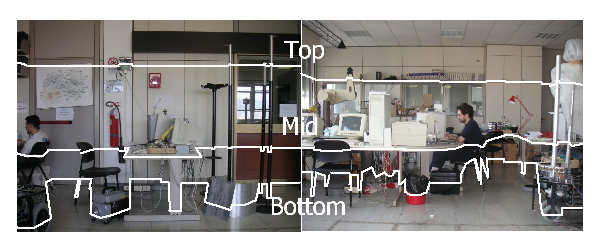
\includegraphics[width=5.0in]{Views}
%\caption{Scan profiles: \emph{bottom}, \emph{mid} and \emph{top view}.}
%\label{fig:views}
%\end{figure}

This is a reference to Figure \ref{fig:views}.

\section{Algorithm} 
\label{sec:algorithm}

This is an algorithm:
\begin{algorithm}
\label{alg:SMS}
\caption{Split \& Merge [\& Split]}
\begin{algorithmic} [1]
\REQUIRE{A scan $s$. A stack $\mathcal{L}$. A counter $j$. A threshold $\tau$}
\ENSURE{$\lambda \leftarrow \mathcal{M}(s)$, $j=1, ..., |\lambda|$}
\STATE{$\mathcal{L}$ = \texttt{push}($s$)}
\STATE{$j \leftarrow 1$}
\WHILE{$\mathcal{L}$ $\neq$ $\varnothing$}
\STATE{$\mathcal{L}$ = \texttt{pop}($s_{top}$)}
\STATE{$l_j$ $\leftarrow$ \texttt{fitting}($s_{top}$)}
\STATE{$q_k = \argmax_{q}\texttt{dist(l$_j$,q)}$}
\IF{$\texttt{dist(l$_j$,$q_k$)} < \tau$}
\STATE{$j \leftarrow j+1$}
\STATE{\texttt{continue}}
\ELSE
\STATE{$s_a \leftarrow$ \texttt{sub}($s_{top}$, 1, $k$)}
\STATE{$s_b \leftarrow$ \texttt{sub}($s_{top}$, $k+1$, $|s|$)}
\STATE{$\mathcal{L}$ = \texttt{push}($s_a$)}
\STATE{$\mathcal{L}$ = \texttt{push}($s_b$)}
\ENDIF
\ENDWHILE
\STATE{\{$l_j$\} $\leftarrow$ \texttt{merge}(\{$l_j$\})}
\STATE{\{$l_j$\} $\leftarrow$ \texttt{split}(\{$l_j$\})}
\end{algorithmic}
\end{algorithm}
%%%%%%%%%%%%%%%%%%%%%%%%%%%%%%%%%%%%%%%%%%%%%%%%%%%%%%%%%%%%%%%%%%%%%%%%%%%%%%%%%
%2345678901234567890123456789012345678901234567890123456789012345678901234567890
%        1         2         3         4         5         6         7         8
% THESIS CONCLUSIONS
%\def\baselinestretch{1}
\chapter{Conclusions}
\label{chap:conclusions}
\ifpdf
    \graphicspath{{Conclusions/Figures/PNG/}{Conclusions/Figures/PDF/}{Conclusions/Figures/}}
\else
    \graphicspath{{Conclusions/Figures/EPS/}{Conclusions/Figures/}}
\fi
%\def\baselinestretch{1.66}

This thesis has presented a kinematic control architecture for two cooperative autonomous underwater manipulators.\\
The robot collaboration is done at kinematic level, exchanging vectors and matrices to produce a common tool Cartesian velocity. The cooperation scheme takes into account that underwater communication is difficult, and it keeps the amount of exchanged data as low as possible.\\
The experimental results showed how the Task Priority Inverse Kinematics approach used can deal with an assembly task: the \textit{peg-in-hole}. Being an unexplored problem for cooperative underwater manipulator, the scenario is simulated with many simplifications and assumptions.\\
Part of the problem deals with computer vision techniques. The thesis shows how some detection and tracking algorithm can be exploited to estimate the hole's pose.\\
For the insertion phase, a force-torque sensor is used to help the accomplishment of the mission, thanks to the data provided exploited by the control architecture.\\
Both the Control and the Vision part can help other works in various robotics fields, not only related to underwater intervention missions.\\

Code implementation is suited to easily manage objectives (e.g. to delete offline some objectives to try a different method). Big effort has been made in providing a modular and flexible code architecture. For example, the dependency from ROS (Robotics Operating System) is kept at minimum to make possible to easily adapt the code to a different kind of interface and/or simulator (which does not rely on ROS to communicate).\\


In the Chapter \ref{chap:introduction}, an introduction about the context is given, and the previous works in the relative fields has been recalled.\\
In Chapter \ref{chap:control}, the principal points of the theory behind the Control Architecture are summarized. Here, the mathematical foundations for the Task Priority Inverse Kinematic approach are recalled, considering also a coordination policy between multiple agents that fits in the chosen approach.\\
In Chapter \ref{chap:method}, the theory explained before is exploited to deal with the scenario stated by this thesis. A Force-Torque objective is inserted in the TPIK list to reduce the magnitudes of forces and torques that act on the peg during the insertion phase. This is noticeable because it is used a \enquote{dynamic} information (the force and the torque) in a pure-kinematic method. A simple, but suitable for the scenario, list of objectives is then described. An additional routine, part not of the kinematic layer but more of the Mission Managing layer, is explained. Considering the goal frame where the peg is driven to by the kinematic control, this new routine shifts its origin according to the direction of the forces acting on the peg. This is an additional method to further exploit the information given by the force-torque sensor.\\
In Chapter \ref{chap:results}, the simulated environment is detailed and the experimental results are discussed. The chosen simulator, UWSim, is introduced, along with some other underwater simulators that can be useful for the interested reader. To make the insertion phase realistic, collisions between the peg and the hole have been inserted in the simulation. These collisions propagates through the whole robotic system, thus affecting the arm and the vehicle. Another routine is implemented to fake a firm grasp of the tool by the two robots. In real environment, this constraint is assured by frictional forces, but in a pure-kinematic simulator like UWSim the frictions are not present. The tuning of the gains permits to not hide bad cooperation between the agents.  In the same Chapter \ref{chap:results}, assumptions to simplify the problem are explained, and an idea of how the Control Loop runs is given. Finally, results of the experiments done are presented and discussed. Three main experiments have been carried out: without hole's pose error, with a fixed error of 0.015m along one axis, and one final test which includes the Vision part with the hole's pose error given by the \textit{Detection} and the \textit{Tracking} algorithms used.\\
Chapter \ref{chap:vision} covers exclusively methods and tools used by the Vision robot. No theoretical background is given because it would take out of the scope of this thesis. The Chapter gives an idea on how two computer vision libraries, \href{https://opencv.org/}{\textbf{OpenCV}} (Open Source Computer Vision Library) [\cite{opencv}] and \href{https://visp.inria.fr/}{\textbf{ViSP}} (Visual Servoing Platform) [\cite{visp}], are used. The Vision part is divided into two phases: Detection and Tracking. For both, different algorithms have been tested, compared and discussed. 
In particular, for the Detection part, some methods have been discarded and they have not been used any more for further trials, but they are anyway presented in Appendix \ref{chap:AppendixVision}. They are all OpenCV algorithms that can help in other applications.\\
This Chapter \ref{chap:conclusions} concludes the thesis and it gives some starting points for possible future works.\\
The Appendix \ref{chap:AppendixCode} gives some details on how the software is implemented, together with a list of some useful libraries used that surely can help to develop a control architecture in the C++ programming language.\\

For some on-going progresses in this scenario, it can be useful for the reader to follow the TWINBOT project [\cite{TWINBOT2019}]. This thesis' context derives from the scenario of this project, but it evolves independently because at the time this thesis was being developed, TWINBOT was in a very early stage.


\section{Future Works}
Since the novelty of the application, further works can be pursued in various directions.\\
For what concerns the experiments, a dynamic simulation, along with a dynamic controller, can be introduced to better analyse the methods adopted. This would mean to include effects that would increase the realism of the simulation, such as buoyancy, thrusters modelling, disturbances of the arm to the vehicle and vice-versa, real tool-grasping effects, even some water currents. Some work has been done in this direction but then it has not been pursued due to the lack of time. These efforts, even if they are not presented in this thesis, showed that the first step to introduce dynamics could be using the plugin \href{https://github.com/freefloating-gazebo/freefloating_gazebo}{FreeFloatingGazebo} [\cite{freeFloatingGazebo}], mentioned in section \ref{sec:simulators}. This one is the most suitable tool to be used from the actual work because its scope is to solve the lack of dynamics of UWSim, expanding the functionalities of the simulator. So, it would be easy to adapt the code to the new simulations. For example, the scene (i.e. the file which describes the simulated scenario) would be the same, and ROS would be always used as interface.\\

Regarding the actual chosen architecture, the Force Torque objective idea can be improved. For example, we can consider a different task reference, calculated not only as a proportional error between the desired force (that is zero) and the actual detected one.\\
Another improvement can be for the Change Goal routine. We could let the forces and the torques modify also the orientation of the goal frame, to reduce/eliminate the angular error between the real goal frame and the one estimated.\\

Regarding the insertion phase, additional problems can be explored. This thesis focused only on collisions that may happen when the peg is already inside the hole. If some contact between the external surface of the hole's structure and the peg's tip happens, the mission fails (i.e., it occurs a stalemate where the peg bounces forever against the hole's surface, unable to find the hole). In the literature, various methods have been explored toward this point. For example, researchers have considered the cases when the peg meets the hole with a bad alignment that creates a two or three points contact (as briefly explained in \ref{sec:artPeg}). However, to the best of this author's knowledge, the \textit{peg-in-hole} problem has never been studied when the protagonists are two autonomous mobile manipulator (in any scenarios, not specifically underwater ones). So, it can be interesting to adapt old tools to this particular (cooperative and underwater) field.\\

Towards a more realistic intervention missions, efforts can be spent to consider ways to localize the robot under the water's surface. In this thesis, it is assumed that all agents have a reference frame in common, but, usually, underwater localization is really an issue. Some cooperative methods (this time not at kinematic level) can be considered to make some surface vessels help the underwater agents to localize themselves (a problem explored in the WiMUST project [\cite{wimust}]).\\

In this thesis, some assumptions have been made for the Vision part. Further works could consider to relax some of them, for example to increase the difficulty of the detection and tracking phases. In an underwater scenario, not always the water permits to watch from afar, and illumination and distortions can be other important issues.\\

There is always a lot of work towards increasing the capacity of \mbox{intervention-AUVs}. For example, we can consider more specifically communication issues and, so, new techniques to exchange data between agents; especially in an underwater scenario, we can't share too much information among robots and with too high frequency. Also, other kinds of assembly problems can be addressed: for instance, a \textit{peg-in-hole} one where the \textit{peg} is held by only one robot and the \textit{hole} by another one.\\ Some objectives of the TWINBOT project [\cite{TWINBOT2019}] aim to study these two just mentioned problems.



\appendix
%%%%%%%%%%%%%%%%%%%%%%%%%%%%%%%%%%%%%%%%%%%%%%%%%%%%%%%%%%%%%%%%%%%%%%%%%%%%%%%%%
%2345678901234567890123456789012345678901234567890123456789012345678901234567890
%        1         2         3         4         5         6         7         8
% THESIS APPENDIX

\chapter{Extra}
\label{chap:appendixA}

Write here...

\bibliographystyle{Classes/RoboticsBiblio}    % bibliography style
\renewcommand{\bibname}{References}           % change default name Bibliography to References
\bibliography{References/references}          % References file
\addcontentsline{toc}{chapter}{References}    % add References to contents page

\end{document}
